
\section{Elektrisches Feld}
\label{section:e_feld}
\begin{frame}%STARTCONTENT

\frametitle{Homogenes elektrisches Feld}
\begin{columns}
    \begin{column}{0.48\textwidth}
    \begin{itemize}
  \item In einem Kondensator wird elektrische Energie gespeichert
  \item Die einfachste Art eines Kondensators ist der \emph{Plattenkondensator}
  \end{itemize}

    \end{column}
   \begin{column}{0.48\textwidth}
       
\begin{figure}
    \DARCimage{0.85\linewidth}{191include}
    \caption{\scriptsize Homogenes Feld in einem Plattenkondensator}
    \label{e_kondensator_homogenes_feld}
\end{figure}


   \end{column}
\end{columns}

\end{frame}

\begin{frame}
\begin{columns}
    \begin{column}{0.48\textwidth}
    \begin{itemize}
  \item An zwei elektrisch leitenden Platten wird jeweils der Plus- und Minus-Pol angeschlossen
  \item Zwischen den Platten baut sich ein homogenes elektrisches Feld (\emph{E-Feld}) auf
  \item Elektrische Feldstärke: $E = \dfrac{U}{d}$ in $\dfrac{V}{m}$
  \item Mit $d$ als Abstand der Platten
  \end{itemize}

    \end{column}
   \begin{column}{0.48\textwidth}
       
\begin{figure}
    \DARCimage{0.85\linewidth}{191include}
    \caption{\scriptsize Homogenes Feld in einem Plattenkondensator}
    \label{e_kondensator_homogenes_feld}
\end{figure}


   \end{column}
\end{columns}

\end{frame}

\begin{frame}
\only<1>{
\begin{PQuestion}{EB101}{Welches Feld stellt sich zwischen zwei parallelen Kondensatorplatten bei Anliegen einer Gleichspannung in Näherung ein?}{Polarisiertes elektrisches Feld}
{Homogenes magnetisches Feld}
{Homogenes elektrisches Feld}
{Polarisiertes magnetisches Feld}
{\DARCimage{1.0\linewidth}{191include}}\end{PQuestion}

}
\only<2>{
\begin{PQuestion}{EB101}{Welches Feld stellt sich zwischen zwei parallelen Kondensatorplatten bei Anliegen einer Gleichspannung in Näherung ein?}{Polarisiertes elektrisches Feld}
{Homogenes magnetisches Feld}
{\textbf{\textcolor{DARCgreen}{Homogenes elektrisches Feld}}}
{Polarisiertes magnetisches Feld}
{\DARCimage{1.0\linewidth}{191include}}\end{PQuestion}

}
\end{frame}

\begin{frame}
\only<1>{
\begin{QQuestion}{EA103}{Welche Einheit wird üblicherweise für die elektrische Feldstärke verwendet?}{Volt pro Meter (V/m)}
{Watt pro Meter (W/m)}
{Ampere pro Meter (A/m)}
{Henry pro Meter (H/m)}
\end{QQuestion}

}
\only<2>{
\begin{QQuestion}{EA103}{Welche Einheit wird üblicherweise für die elektrische Feldstärke verwendet?}{\textbf{\textcolor{DARCgreen}{Volt pro Meter (V/m)}}}
{Watt pro Meter (W/m)}
{Ampere pro Meter (A/m)}
{Henry pro Meter (H/m)}
\end{QQuestion}

}
\end{frame}

\begin{frame}
\only<1>{
\begin{QQuestion}{EB102}{An einem Plattenkondensator mit \qty{0,6}{\centi\metre} Plattenabstand werden \qty{9}{\volt} angelegt. Wie groß ist die elektrische Feldstärke zwischen den beiden Platten näherungsweise?}{\qty{5,4}{\V}/m}
{\qty{150}{\V}/m}
{\qty{540}{\V}/m}
{\qty{1500}{\V}/m}
\end{QQuestion}

}
\only<2>{
\begin{QQuestion}{EB102}{An einem Plattenkondensator mit \qty{0,6}{\centi\metre} Plattenabstand werden \qty{9}{\volt} angelegt. Wie groß ist die elektrische Feldstärke zwischen den beiden Platten näherungsweise?}{\qty{5,4}{\V}/m}
{\qty{150}{\V}/m}
{\qty{540}{\V}/m}
{\textbf{\textcolor{DARCgreen}{\qty{1500}{\V}/m}}}
\end{QQuestion}

}
\end{frame}

\begin{frame}
\frametitle{Wickelkondensator}
\begin{columns}
    \begin{column}{0.48\textwidth}
    \begin{itemize}
  \item Bei einem Wickelkondensator wird zwischen den beiden Platten als Metallbeläge ein Isolator als \emph{Dielektrikum} eingebracht
  \item Vorteile: platzsparend und größere Plattenfläche möglich
  \end{itemize}

    \end{column}
   \begin{column}{0.48\textwidth}
       
\begin{figure}
    \DARCimage{0.85\linewidth}{49include}
    \caption{\scriptsize Schematische Darstellung eines Wickelkondensators}
    \label{e_wickelkondensator}
\end{figure}


   \end{column}
\end{columns}

\end{frame}

\begin{frame}
\only<1>{
\begin{PQuestion}{EB103}{An den Metallbelägen eines Wickelkondensators mit \qty{0,15}{\mm} starkem Kunststoff-Dielektrikum liegt eine Spannung von \qty{300}{\V}. Wie hoch ist die elektrische Feldstärke zwischen den Metallbelägen ungefähr?}{\qty{2000}{\V}/m}
{\qty{200}{\V}/m}
{\qty{2000}{\kV}/m}
{\qty{200}{\kV}/m}
{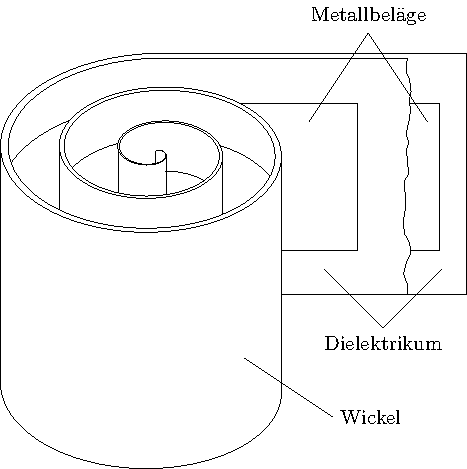
\includegraphics[width=1.0\linewidth]{img/49.pdf}}\end{PQuestion}

}
\only<2>{
\begin{PQuestion}{EB103}{An den Metallbelägen eines Wickelkondensators mit \qty{0,15}{\mm} starkem Kunststoff-Dielektrikum liegt eine Spannung von \qty{300}{\V}. Wie hoch ist die elektrische Feldstärke zwischen den Metallbelägen ungefähr?}{\qty{2000}{\V}/m}
{\qty{200}{\V}/m}
{\textbf{\textcolor{DARCgreen}{\qty{2000}{\kV}/m}}}
{\qty{200}{\kV}/m}
{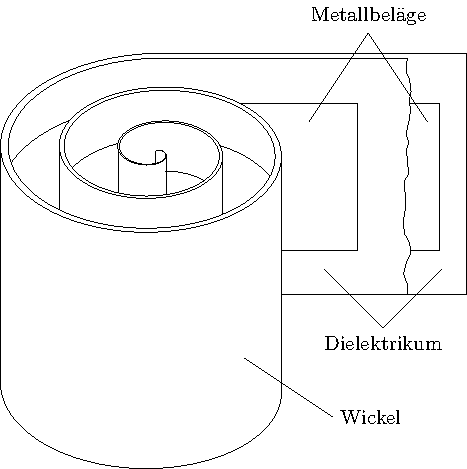
\includegraphics[width=1.0\linewidth]{img/49.pdf}}\end{PQuestion}

}
\end{frame}

\begin{frame}
\only<1>{
\begin{QQuestion}{EB104}{Ein Kondensator in einer Senderendstufe hat eine \qty{0,15}{\mm} starke PTFE-Folie als Dielektrikum. Die Durchschlagsfestigkeit von PTFE beträgt ca. \qty{400}{\kV}/cm. Wie groß wäre die maximale Spannung, die an den Kondensator angelegt werden kann, ohne dass die Folie durchschlagen wird?}{\qty{26}{\V}}
{\qty{60}{\kV}}
{\qty{6}{\kV}}
{\qty{2,6}{\kV}}
\end{QQuestion}

}
\only<2>{
\begin{QQuestion}{EB104}{Ein Kondensator in einer Senderendstufe hat eine \qty{0,15}{\mm} starke PTFE-Folie als Dielektrikum. Die Durchschlagsfestigkeit von PTFE beträgt ca. \qty{400}{\kV}/cm. Wie groß wäre die maximale Spannung, die an den Kondensator angelegt werden kann, ohne dass die Folie durchschlagen wird?}{\qty{26}{\V}}
{\qty{60}{\kV}}
{\textbf{\textcolor{DARCgreen}{\qty{6}{\kV}}}}
{\qty{2,6}{\kV}}
\end{QQuestion}

}
\end{frame}

\begin{frame}
\frametitle{Lösungsweg}
Der Trick ist hier, dass die Durschlagsfestigkeit die elektrische Feldstärke $E$ ist.

\begin{itemize}
  \item Gegeben: $d = 0,15mm$ und $E = 400\frac{kV}{cm}$
  \item Gesucht: $U$
  \item Lösung:
  \end{itemize}
$E = \frac{U}{d} \Rightarrow U = E\cdot d$

$U = 400\cdot\frac{10^3V}{10^{-2}m}\cdot 0,15\cdot 10^{-3}m$

$U = 6\cdot10^3V = 6kV$

\end{frame}

\begin{frame}
\frametitle{Vertikalantenne}
\begin{columns}
    \begin{column}{0.48\textwidth}
    \begin{itemize}
  \item An einer Antenne entstehen ebenso elektrische Feldlinien
  \item Die Feldlinien einer Vertikalantenne verlaufen vom \enquote{positiven Ende} zur Erde
  \end{itemize}

    \end{column}
   \begin{column}{0.48\textwidth}
       
\begin{figure}
    \DARCimage{0.85\linewidth}{193include}
    \caption{\scriptsize Feldlinien an einer Vertikalantenne}
    \label{e_feldlinien_vertikalantenne}
\end{figure}


   \end{column}
\end{columns}

\end{frame}

\begin{frame}
\only<1>{
\begin{PQuestion}{EB105}{Wie werden die mit X gekennzeichneten Feldlinien einer Vertikalantenne bezeichnet?}{Radiale Feldlinien}
{Magnetische Feldlinien}
{Elektrische Feldlinien}
{Horizontale Feldlinien}
{\DARCimage{1.0\linewidth}{193include}}\end{PQuestion}

}
\only<2>{
\begin{PQuestion}{EB105}{Wie werden die mit X gekennzeichneten Feldlinien einer Vertikalantenne bezeichnet?}{Radiale Feldlinien}
{Magnetische Feldlinien}
{\textbf{\textcolor{DARCgreen}{Elektrische Feldlinien}}}
{Horizontale Feldlinien}
{\DARCimage{1.0\linewidth}{193include}}\end{PQuestion}

}
\end{frame}%ENDCONTENT
